\begin{figure}[t]
    \centering
    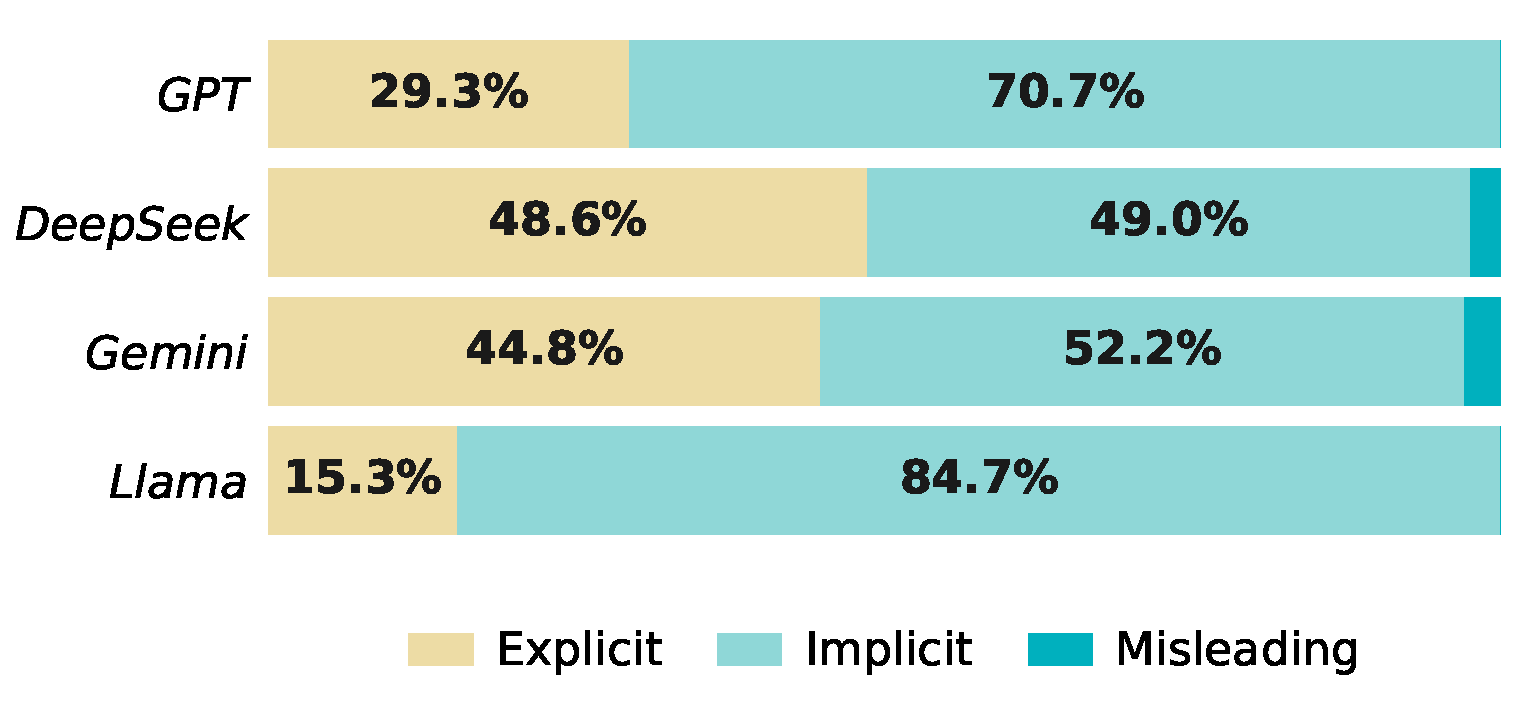
\includegraphics[width=1\linewidth]{Figures/noisy_tool_behavior_inner_bar.pdf}
    \vspace{-0.35in}
    \caption{Distribution of invoked block alternatives under \textit{mixed} blocking. For each model, the horizontal bar normalizes all invoked block alternatives to $100\%$. Colors indicate whether the invoked block alternative is an explicit failure, implicit failure, or semantic misleading tool. We abbreviate \textit{GPT-5.4}, \textit{Gemini-3.5-Flash}, \textit{DeepSeek-V4-Flash}, and \textit{Llama-3.3-70B-Instruct} as \textit{GPT}, \textit{Gemini}, \textit{DeepSeek}, and \textit{Llama}.}
    \label{fig:noisy_tool_type_mix}
    % \vspace{-0.2in}
\end{figure}